% Build with `pdflatex slides.tex`
\documentclass[xcolor=pdftex,dvipsnames,table]{beamer}

\mode<presentation> {
  \usetheme{Warsaw}
  \setbeamercovered{transparent}
%  \useoutertheme{infolines}
%  \setbeamertemplate{headline}[default]
%  \setbeamertemplate{footline}[infolines theme]{}
}

\usepackage{hyperref}
\usepackage[english]{babel}

\usepackage[latin1]{inputenc}

\usepackage{times}
\usepackage[T1]{fontenc}

\usepackage{amssymb}

\usepackage{ulem}

\usepackage{overpic}
\usepackage{color}

\hypersetup{%
    pdftitle={Characterising User Interactivity for Sports Video-on-Demand},
    pdfauthor={Andrew Brampton, Andrew MacQuire, Idris A. Rai, Nicholas J. P. Race, Laurent Mathy and Michael Fry},
    pdfkeywords={Interactive, Sports, Video-on-Demand, Worldcup, Content Distribution},
    bookmarksnumbered,
    pdfstartview={FitH},
    colorlinks=false,
    linkcolor={black},%: Color for normal internal links.
    anchorcolor={black},%: Color for anchor text.
    citecolor={black},%: Color for bibliographical citations in text.
    filecolor={black},%: Color for URLs which open local files.
    menucolor={black},%: Color for Acrobat menu items.
    pagecolor={black},%: Color for links to other pages
    urlcolor={black}%: Color for linked URLs.
}

\title[Interactive Sports Video-on-Demand]
{\textbf{Characterising User Interactivity for Sports Video-on-Demand}}

\institute[Lancaster University, UK] {
    \href{mailto:brampton@comp.lancs.ac.uk}{\textbf{Andrew Brampton}},
    \href{mailto:macquire@comp.lancs.ac.uk}{Andrew MacQuire},
    \href{mailto:rai@comp.lancs.ac.uk}{Idris Rai},
    \href{mailto:race@comp.lancs.ac.uk}{Nicholas Race},
    \href{mailto:laurent@comp.lancs.ac.uk}{Laurent Mathy}
     (Lancaster University, UK)\\and\\

    \href{mailto:michael.fry@usyd.edu.au}{Michael Fry}
     (The University of Sydney, AU)\\~\\

    \{\href{mailto:brampton@comp.lancs.ac.uk}{brampton},
    \href{mailto:macquire@comp.lancs.ac.uk}{macquire},
    \href{mailto:rai@comp.lancs.ac.uk}{rai},
    \href{mailto:race@comp.lancs.ac.uk}{race},
    \href{mailto:laurent@comp.lancs.ac.uk}{laurent}\}
    @comp.lancs.ac.uk {\it and}
    \href{mailto:michael.fry@usyd.edu.au}{michael.fry@usyd.edu.au}

}

\date[5th June 2007]
{Tuesday 5th June \\ \textbf{NOSSDAV 2007}}

\subject{Characterising User Interactivity for Sports Video-on-Demand}

\logo{
\includegraphics[height=0.85cm]{uni-logo-win}}

\setbeamertemplate{navigation symbols}{}

%\renewcommand{\textbf}{\alert}

\begin{document}

\begin{frame}
  \titlepage
\end{frame}

\section{Introduction}

\begin{frame}
    \frametitle{Outline}
    {\small
        \tableofcontents
    }
\end{frame}

\begin{frame}
    \frametitle{Introduction}
    % Talk about what I will show in this talk,
    % explain we used a popular media (Worldcup)
    % state that what we have seen is different to what's been seen in the past

    \textbf{Characterising User Interactivity for Sports Video-on-Demand}
    \begin{itemize}
        \item Created a simple Video-on-Demand service offered to university staff and students~\\

        \item Served interactive sport videos (specifically 2006 FIFA World Cup)~\\

        \item Obtained traces and characterised the interactive user behaviour~\\

        \item Interactivity has an dramatic impact~\\
        \item Discuss how Content Distribution Networks (CDNs) can exploit this behaviour~\\
    \end{itemize}
\end{frame}

%\begin{frame}
%    \frametitle{Introduction (idea 2 - I will show this slide, OR prev)}
%
%    \center{\it\small
%        This paper presents a \textbf{detailed characterisation} of user behaviour
%        for a series of \textbf{interactive sport videos} from the 2006 \textbf{FIFA World
%        Cup}. In addition to generic VCR-like features, our custom-built
%        \textbf{Video-on-Demand} architecture enabled us to provide advanced
%        interactivity features such as \textbf{bookmarking}. We illustrate how such
%        functionality may have a dramatic impact on how users consume
%        content. A detailed \textbf{discussion} is also provided on how \textbf{content
%        distributors} may turn this knowledge to their advantage, and thus
%        \textbf{increase} the \textbf{efficiency} of their \textbf{delivery networks}.
%    }
%\end{frame}

\subsection{Motivation}

\begin{frame}
    \frametitle{Motivation 1}
    % Reading out and expanding what's listed on the slide :)

    \begin{itemize}
        \item Increase in the use of \textbf{bandwidth intense streaming} videos~\\~\\
        \item Users expect \textbf{more interactivity} (VCR, Bookmarks, Time-shifting)~\\~\\

        \item Content Distribution Networks are used to alleviate these problems
        \begin{itemize}
            \item \textbf{Need to know workloads} to exploit behaviour (caching, replication, streaming protocols)
        \end{itemize}~\\

    \end{itemize}
\end{frame}

\begin{frame}
    \frametitle{Motivation 2}
    % Reading out and expanding what's listed on the slide :)

    \begin{itemize}
        \item Traditional workloads are \textbf{not very interactive}
        \begin{itemize}
            \item Simple start-to-finish models
            \item Only minimal VCR interactivity
            \item \textbf{Never considered bookmarks}
        \end{itemize}~\\

        \item Large traces are private~\\~\\
        \item Publicly available traces are \textbf{non-interactive and/or outdated}.~\\~\\
        \item Previous work \textbf{hasn't looked at sports} in particular~\\~\\
    \end{itemize}
\end{frame}

\subsection{Related Work}

\begin{frame}
    \frametitle{Related Work}
    % Non-interactive analysis - Looking at arrive rates, session times, popularity, etc
    % [1] Looks at what kind of streaming is happening today (however a lot has changed in 3 years)
    % [2] Large VoD service (from China Telecom), User interests change over time, arrival rates and session times.

    % Interactive - Look at similar metrics as the previous papers, but also looks at the # of VCR style requests,
    %               and distance jumped etc. But little more analysis, some of which contradicts our results.
    % [3] Education (and some Entertainment), Found pause to be most common, also says File segments are uniformly accessed
    % [4] Looks at Spanish news website, State the number of VCR requests

%    \textbf{Static}
%    \begin{itemize}
%        % Looks at what kind of streaming is happening today
%        \item Sripanidkulchai~{\it et al}. An analysis of live streaming workloads on the Internet. 2004.
%
%        % Large VoD service (from China Telecom), User interests change over time, arrival rates and session times.
%        \item Yu~{\it et al}. Understanding user behavior in large scale video-on-demand systems. 2006.
%    \end{itemize}~\\
%
%    \textbf{Interactive}
%    \begin{itemize}
%        % Education (and some Entertainment), Found pause to be most common
%        \item Costa~{\it et al}. Analyzing client interactivity in streaming media. 2004.
%
%        % Looks at Spanish news website, State the number of VCR requests
%        \item Vilas~{\it et al}. User Behaviour Analysis of a Video-On-Demand Service with a Wide Variety of Subjects and Lengths. 2005.
%    \end{itemize}

    {\footnotesize

        % Looks at what kind of streaming is happening today using Akami traces
        An analysis of live streaming workloads on the Internet. Sripanidkulchai~{\it et al}\\
        % Large VoD service (from China Telecom), User interests change over time, arrival rates and session times.
        Understanding user behavior in large scale video-on-demand systems. Yu~{\it et al}
        \begin{itemize}
            \item Looks at what kind of streaming is happening today (2004)
            \item Looks at metrics such as arrival rates and session times
        \end{itemize}~\\

        % Education (and some Entertainment), Found pause to be most common
        Analyzing client interactivity in streaming media. Costa~{\it et al}
        \begin{itemize}
            \item Looks at \textbf{simple VCR} (fast forward/rewind/pause)
            \item \textbf{Only education} and some entertainment
        \end{itemize}~\\

        % Looks at Spanish news website, State the number of VCR requests
        User Behaviour Analysis of a Video-On-Demand Service with a Wide Variety of Subjects and Lengths. Vilas~{\it et al}
        \begin{itemize}
            \item Again only has simple VCR
            \item Mostly short news videos on a wide range of subjects
        \end{itemize}~\\

    }

\end{frame}

\subsection{Experiment Setup}

\begin{frame}
    \frametitle{Video-on-Demand System Setup}
    % To collect our results we needed to setup a system. Explain the system, and mention it's available online

    \begin{center}
        \includegraphics[width=10.75cm]{../NOSSDAV07/diagrams/setup}
        \\Source code available at: www.rcdn.org
    \end{center}

\end{frame}

\begin{frame}
    \frametitle{Player Interface}

    % Explain what features the interface had,
    % Make clear that the forward/backward buttons don't speed up/slow down, but instead jump
    % Say that it does influence results, but this can't be helped
    % Justify why we used each control

    \begin{center}

        \begin{overpic}[width=10cm] {../NOSSDAV07/diagrams/InterfaceEdit}
            \color{red}
            \linethickness{2pt}
            \only<2> { \put (0,8){ \framebox(85.5,47) } }
            \only<3> { \put (0,0){ \framebox(86,7) } }
            \only<4> { \put (86,0){ \framebox(13,56) } }
        \end{overpic}
%        \only<1>{}
%        \only<2>{Main Player Area}
%        \only<3>{Controls} % - Seek bar, Forward (10,30,60), Back (10,30,60), Pause/Resume, Tag}
%        \only<4>{Bookmarks} % - Main bookmarks, User Bookmarks}
    \end{center}

\end{frame}


\section{Analysis}

\begin{frame}
    \frametitle{Methodology}

    % Briefly mention the stats, and re-state that we did this analysis to characterise the
    % interactive nature of the media, and to aid in simulating and creating new protocols.

    % Andy suggests we remove the amount of users

    \textbf{Results}
    \begin{itemize}
        \item 66 matches (64 Worldcup matches, and 2 pre-competition friendlies)
        \item 13$^{th}$ June until 16$^{th}$ July 2006
        \item 405 unique users, average 30.7 users per game
    \end{itemize}~\\

    \textbf{Models}
    \begin{itemize}
        \item Fitted models (where appropriate)
        \item Helps to understand the nature of the result
        \item Allows future simulations to use models
    \end{itemize}

\end{frame}


\subsection{Popularity}

\begin{frame}
    \frametitle{Argentina vs. Serbia and Montenegro viewers}
    % This shows the popularity of different 1 second segments of a particular match
    % Areas around bookmarks are more popular
    % The majority of the video only got ~10%, whereas the hotspots had 50% and above
    % Different to previous results where the media was uniformly popular.
    % Also bookmark hint to where will be popular, and could be useful for replication

    \begin{overpic}[width=10cm] {arg-scg_views_normal}
        \color{blue}
        \only<2> {
            \put (53,42){ \vector(-1, 1){10} }
            \put (53,40){ \footnotesize Peaks of interest }
        }
        %\only<2> { \put (20,30){ \circle{50} } }
    \end{overpic}

    {\footnotesize
    \begin{itemize}
        \item {Most of the video was equally popular, with peaks of high interest around bookmarks}
    \end{itemize}
    }

    %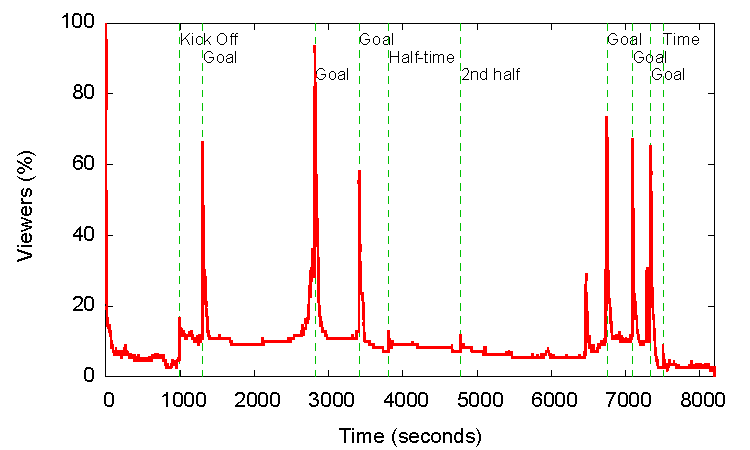
\includegraphics[width=11cm]{../diagrams/arg-scg_views_normal}

\end{frame}

\begin{frame}
    \frametitle{Object and Segment Popularity}
    % Expanding from the previous graph, this shows a CDF of the popularity of the matchs (listed as objects)
    % and the 1 second segments.
    % We can see this follows a power-law distribution, with some segments being very popular
    % complete departure from previous results that show a roughly uniform popularity of the whole video
    % emphasises the need for segment caching,
    % Object popularity follows a simple normal distribution, Previously results have show a Zipf, however
    % we have small number of videos, and videos were generally only popular for a couple of days

    \includegraphics[width=10cm]{../NOSSDAV07/diagrams/all_sessions_rank}

    {\footnotesize
    \begin{itemize}
        \item {Segment popularity exhibits Power-law distribution}
    \end{itemize}
    }

\end{frame}

\subsection{Interactivity}

\begin{frame}
    \frametitle{Occurrences of interactive actions}
    % This table is slightly different to the one in the paper, also shows totals
    % Shows how often each kind of control was used
    % Notice the high number of bookmark usage
    % Forwards also very popular
    % The next slide will help us understand when different actions are being used
    % Useful to know so the network can be designed to cope

    {\small
    \begin{tabular}{|c|c|c|c|}
        \hline
        Action & Occurrences & Percentage(\%) & per Session\\
        \hline

        Back 10s        & 1353 & 5.98  & 0.58 \\
        Back 30s        & 556  & 2.46  & 0.24 \\
        Back 60s        & 775  & 3.43  & 0.33 \\
        Forward 10s     & 3319 & 14.67 & 1.42 \\
        Forward 30s     & 1664 & 7.36  & 0.71 \\
        Forward 60s     & 3488 & 15.42 & 1.49 \\
        Seek-bar        & 2101 & 9.29  & 0.90 \\
        Bookmarks       & 5203 & 23.00 & 2.22 \\
        User bookmarks  & 585  & 2.59  & 0.25 \\

        Add bookmark    & 43   & 0.19  & 0.02 \\
        Pause           & 1847 & 8.16  & 0.79 \\ % There was 103 "double" pauses
        Resume          & 1690 & 7.47  & 0.72 \\ % There was 866 resumes pressed needlessly

        \hline\hline

        Total Back     & 2684 & 11.87 & 1.15 \\
        Total Forward  & 8471 & 37.45 & 3.62 \\
        Total Seeks    & 19044 & 84.2 & 8.14 \\

        \hline
        \end{tabular}
    }

\end{frame}

\begin{frame}
    \frametitle{Argentina vs. Serbia and Montenegro jumps}
    % Shows where people sought within the video, and from where
    % give an example (to clarify plot)
    % Point out clusters of points and explain what they mean (ie shortly after a bookmark, people jump to another bookmark) From 1300 to 2900, and then 2900 to 3500
    % Lack of points on the diagonal,
    %    ones that exist are above line between bookmarks
    % OR below line around bookmark (indicates re-watching)
    % This is all useful, because it helps us to know what to cache and could make user behaviour predictable

    \begin{overpic}[width=10cm] {arg-scg_jumps}
        \color{blue}
        \only<2> {
            \put (48, 42){ \vector(-1, 1) {5} }
            \put (48, 42){ \footnotesize Jumped from 2900 seconds to 6800 seconds }
        }
        \only<3> {
            \put (28,26){ \circle{5} }
            \put (43,30){ \circle{5} }
            \put (30,26){ \footnotesize Clusters of jumps }
        }
        \only<4> {
            \put (48, 21){ \vector(-1, 1) {5} }
            \put (48, 21){ \footnotesize Back jumps around a bookmark }
        }
    \end{overpic}

    {\footnotesize
    \begin{itemize}
        \item {Clusters of jumps (indicates users followed similar patterns)}
        \item {Small Forward and Back jumps occur in certain areas}
    \end{itemize}
    }

\end{frame}

\begin{frame}
    \frametitle{CDF of session lengths and inter-seek times}
    % Shows session time - defined as the time between a user visited a video and eventually leaving
    % Interseek time - defined the duration a user watched before seeking (or leaving the video)

    % max video was ~ 10,000 seconds long - Therefore some paused the video (and came back a lot later)
    %   follows normal session times

    % 90% of inter-seek times were <100seconds. A lot shorter than previous workloads.
    % 60% < 10seconds Indicates lots of seeking

    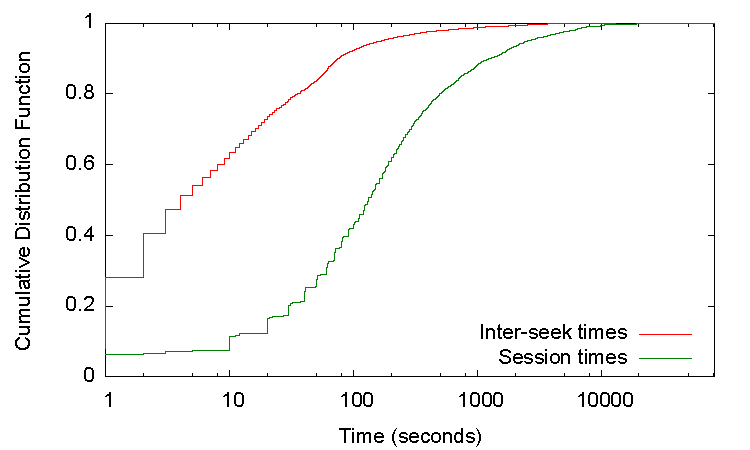
\includegraphics[width=10cm]{view_user_sessions_cdf}

    {\footnotesize
    \begin{itemize}
        \item {Short time between seeks}
        \item {Majority of sessions are a lot shorter than the media length}
    \end{itemize}
    }

\end{frame}

\section{Outlook}
\subsection{Outlook}

\begin{frame}
    \frametitle{Outlook}
    % Explain what's next, now that we have a characterisation.
    % Talk about each of the following points

    \textbf{Characterising}
    \begin{itemize}
        \item Confirm these results apply to other types of video content
        \item Other sports, music, news
    \end{itemize}~\\

    Create \textbf{protocols/algorithms} to exploit these characterisations:
    \begin{itemize}
        \item Segmentation
        \begin{itemize}
            \item 60\% of requests < 10 seconds long
        \end{itemize}

        \item Bookmarks
        \begin{itemize}
            \item Caching / replication should exploit them
            \item Automatic positioning (or repositioning)
        \end{itemize}

    \end{itemize}
\end{frame}

\begin{frame}
    \frametitle{Outlook - Bookmarks Misplacement}
    % Explain that the graph shows ~6-8\% of bookmarks might have been misplaced, this is because
    % users sought before, or after the bookmark. Also mention about the penalties, and how
    % most (if not all) had users seeking around them.

    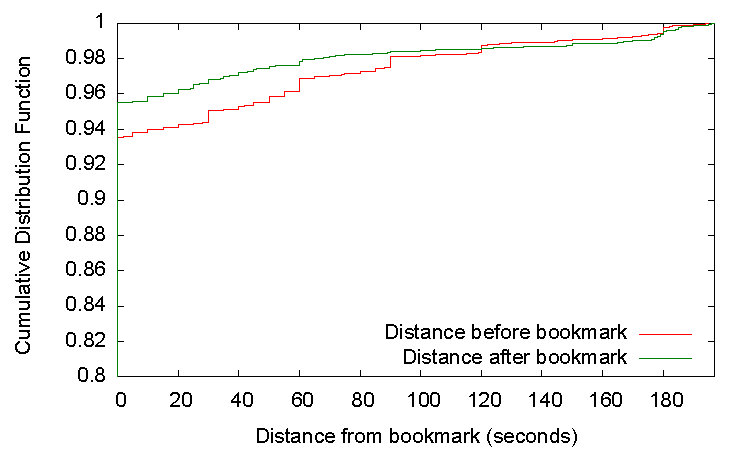
\includegraphics[width=10cm]{all_backs_cdf-20}

    {\footnotesize
    \begin{itemize}
        \item {93\% - 95\% of the time users did not seek after visiting a bookmark}
        \item {Therefore 5\% - 8\% of bookmarks were misplaced}
    \end{itemize}
    }

\end{frame}

\begin{frame}
    \frametitle{Outlook}
    % Explain that users generally followed the same sequence of bookmarks,
    % This would all a CDN to prefetch or prepush content to the user before its request
    % To test this we divided the sequence of events in sequence pairs (as illustrated)

    \textbf{Prediction}
    \begin{itemize}
        \item Users watched bookmarks in a similar order
        \item Pre-fetch/Pre-push bookmark before it is requested
    \end{itemize}

    \textbf{Sequence of bookmarks:}
%    \only<1>{Start -> Kick Off -> Goal 1-0 -> Goal 1-1 -> End}
%    \only<2>{\textbf{(Start -> Kick Off)} -> Goal 1-0 -> Goal 1-1 -> End}
%    \only<3>{Start -> \textbf{(Kick Off -> Goal 1-0)} -> Goal 1-1 -> End}
%    \only<4>{Start -> Kick Off -> \textbf{(Goal 1-0 -> Goal 1-1)} -> End}
%    \only<5>{Start -> Kick Off -> Goal 1-0 -> \textbf{(Goal 1-1 -> End)}}
    \begin{center}
        \includegraphics[width=7cm]{sequence}
    \end{center}
\end{frame}


\begin{frame}
    \frametitle{Outlook - Prediction}
    % Explain how this graph is the CDF of the sequence pair,
    % State that over 20\% of the pairs have a 50\% probability of occurring. This means there are many
    % events we can predict with high accuracy that a user will take.

    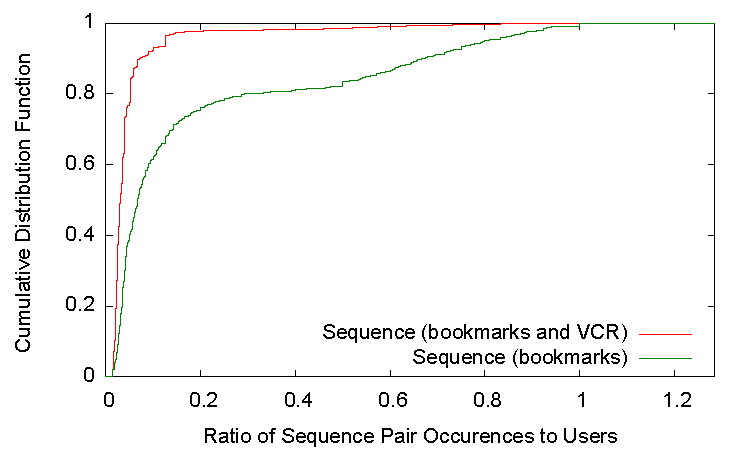
\includegraphics[width=10cm]{all_sequence_normal_cdf}

    {\footnotesize
    \begin{itemize}
        \item {Top 20\% bookmark sequence occur 50\% of the time}
        \item {Sequences with VCR is less predictable}
    \end{itemize}
    }

\end{frame}

\subsection{Conclusion}

\begin{frame}
    \frametitle{Conclusion}
    % Just summaries the talk with the points on the slides

    \begin{itemize}
        \item Created a interactive VoD service (with the 2006 FIFA Worldcup)~\\~\\

        \item Characterised interactive user behaviour~\\~\\

        \item Interactivity highly influences users~\\
        \begin{itemize}
            \item Bookmarks leads to access patterns not previously seen
        \end{itemize}~\\

        \item Content Distribution Networks can exploit this behaviour~\\~\\
    \end{itemize}

\end{frame}

\begin{frame}

    % blank the date, so the last frame fits on properly
    \date[] {}

    %\frametitle{Thank you for listening}
    \begin{center}
        \textbf{Thank you for listening\\Any questions?\\}
        \titlepage
    \end{center}
\end{frame}

% What addition slides could I place here (as backup + extra time)

\end{document}
